%
%
%
%%%%%%%%%%%%%%%%%%%%%%%%%%%%%%%%%%%%%%%%%%%%%%%%%%%%%%%%%%%%%%%%%%%%%%%
%                           SUBSUBSECTION                             %
%%%%%%%%%%%%%%%%%%%%%%%%%%%%%%%%%%%%%%%%%%%%%%%%%%%%%%%%%%%%%%%%%%%%%%%
%
%
%

\subsection{Спектральная плотность энергии. Формула Планка}

    К построению кривой спектральной плотности энергии $u(\omega)$ будем подходить методами статистики через количество фотонов с данной энергией в единице объема пространства.

    Фотоны подчиняются статистике Бозе-Эйнштейна, потому для среднего числа частиц с данной энергией $\varepsilon = \hbar \omega$ справедливо
    %
    \begin{equation}
        n(\varepsilon) = \frac{1}{\exp(\flatfrac{\varepsilon}{kT}) - 1} .
    \end{equation}
    %
    Спектральная плотность энергии может быть выражена как
    %
    \begin{equation}\label{eq:psd}
        u(\omega) \dd{\omega} = \hbar\omega\ n(\hbar\omega) \dd{N(\omega)} ,
    \end{equation}
    %
    где $N(\varepsilon)$~--- число мод электромагнитного поля в единице объема пространства с частотами в бесконечно малой окрестности $\omega$. Таким образом, для получения $u(\omega)$ необходимо лишь знать вид $\dv*{N}{\omega}$.

    Можно показать \cite{sivuhin_opt}, что число стоячих волн с частотами $[\omega,\omega+\dd{\omega}]$ в единице объема трехмерного пространства асимптотически ($\omega \to \infty$) распределено в соответствии с законом
    %
    \begin{equation}\label{eq:dN_of_eps_cont}
        \dd{N(\omega)} = \frac{\omega^2 \dd{\omega}}{\pi^2 v^3} .
    \end{equation}
    %
    Как и ранее, $v$ здесь обозначает скорость света в среде. При подстановке \autoref{eq:dN_of_eps_cont} в \autoref{eq:psd} спектральная плотность энергии $u(\omega)$ приобретает известный вид:
    %
    \begin{equation}
        u(\omega) = \frac{
                \flatfrac{\omega^2 \hbar\omega}{\pi^2 v^3}
        }{\exp(\flatfrac{\hbar\omega}{kT}) - 1} .
    \end{equation}
    %
    Это знаменитая формула Планка, полученная им для излучения абсолютно черного тела.

%
%
%
%%%%%%%%%%%%%%%%%%%%%%%%%%%%%%%%%%%%%%%%%%%%%%%%%%%%%%%%%%%%%%%%%%%%%%%
%                           SUBSECTION                                %
%%%%%%%%%%%%%%%%%%%%%%%%%%%%%%%%%%%%%%%%%%%%%%%%%%%%%%%%%%%%%%%%%%%%%%%
%
%
%

\subsection{Построение кривой спектральной плотности энергии}

    Перейдем к непосредственному построению спектральной плотности энергии поля в резонаторе.

    Ранее было показано, что собственные частоты резонатора $\omega_n$ определяется нулями радиальных частей сферических мод. Известно, что радиальная часть моды зависит только от $l$ и не зависит от $m \in \qty[-l,l]$. Следовательно, $l$-я мода является $2l + 1$-вырожденной по энергии.

    Будем обозначать собственные частоты, полученные из граничных условий для $p$-поляризованной $l$-й моды, как $\omega^{lp}_n$, т.е. снабдим существующий набор $\omega_n$ дополнительными индексами. Будем также для удобства предполагать, что $\omega_n$ упорядочены по $n$: всегда выполняется $\omega_{n-1} \le \omega_n$. В таких обозначениях некоторой данной $\omega^{lp}_n$ соответствует $2l + 1$ мода с фиксированным $l$ и различными $m$.

    Дальнейшая наша задача на пути к построению асимптотической кривой спектральной плотности энергии сводится к следующему. Необходимо показать, что и в случае сферического резонатора наблюдается асимптотическое поведение $\dv*{N}{\omega} \sim \omega^2$ при больших $\omega$. Для этого необходимо посчитать $\dv*{N}{\omega} \approx \flatfrac{\Delta N}{\Delta \omega}$ по существующему спектру мод, т.е. фактически произвести свертку функции дискретного аргумента $N(\omega^{lp}_n) = 2l + 1$ с окном $\Delta \omega$.

    Изобразим функцию $N(\omega_n)$ (\autoref{fig:n}). Каждая \enquote{строчка} функции соответствует аргументам $\omega^{lp}_i$ для обеих значений $p$ и фиксированного значения $l$. Численно $\omega^{lp}_i$ являются нулями радиальных функций. С увеличением $l$ независимо от поляризации увеличивается также и положение самого левого нуля радиальной функции. Нули радиальных функций обеих поляризаций находятся близко друг к другу. Асимптотически при $i \to \infty$ расстояние между соседними нулями каждой из радиальных функций стремится к $\pi$.
    %
    \begin{figure}[h]
        \centering
        %
        \subfloat[][]{%
            \label{fig:n_all}%
            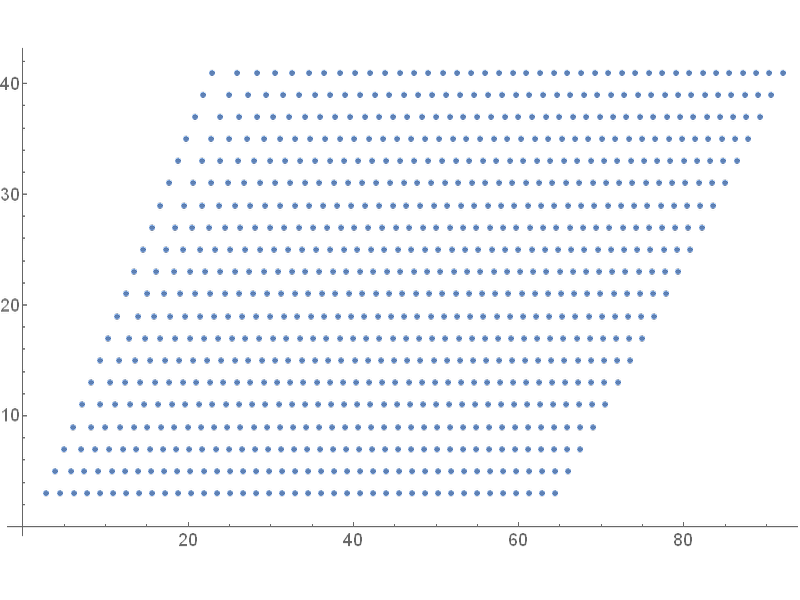
\includegraphics[width=0.45\textwidth]{n}}%
        \hspace{8pt}%
        %
        \subfloat[][]{%
            \label{fig:n_full}%
            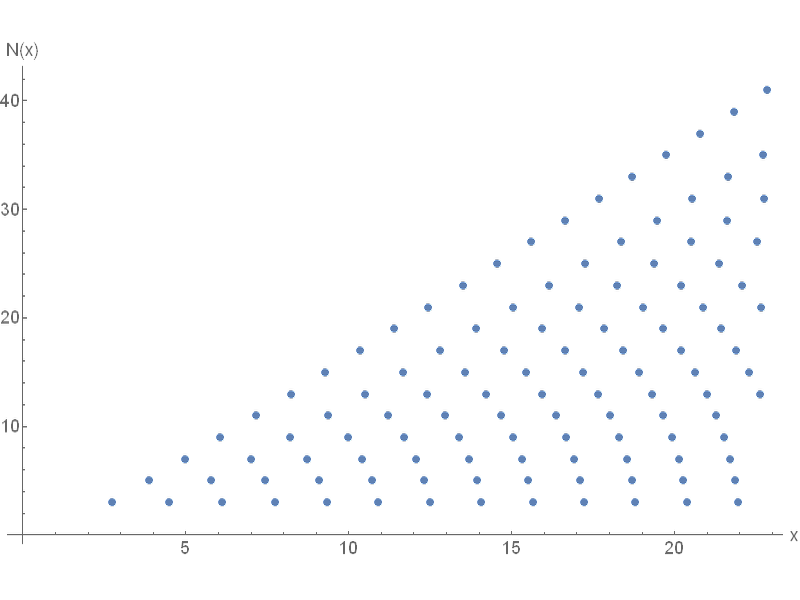
\includegraphics[width=0.45\textwidth]{n_full}}%
        \hspace{8pt}%
        %
        \caption[]{Функция $N(\omega_n)$ (аргумент в относительных единицах). Параметр $l_{max} = 300$. На \subref{fig:n_full} увеличена область $\omega < \Omega$. %
        } %
        \label{fig:n}%
    \end{figure}

    Описанная картина говорит о следующем. Пусть мы имеем некоторый рассчитанный конечный набор $\omega^{lp}_n$, $n = 1, 2, \dots, n_{max}$, полученный из $2 * (l_{max} - l_{min})$ различных базовых мод (двойка соответствует числу возможных поляризаций). В области $0 < \omega \le \Omega = \min_p{\omega^{l_{max}p}_{i_{min}}}$, где $i_{min}$~--- индекс самого левого нуля $l_{max}$-й радиальной функции $p$-й поляризации, имеется полная информация о функции $N(\omega_n)$. Иными словами, в этой области она построена по всем своим возможным аргументам. В области $\omega > \Omega$ отсечены значения функции $N(\omega^{lp}_n)$ с $l > l_{max}$, потому она не пригодна для дальнейшего рассмотрения. Под $l_{min}$ здесь понимается минимальное физически возможное значение $l$. Ранее было показано, что $l_{min} = 1$.

    На \autoref{fig:dndx} изображена функция $\flatfrac{\Delta N}{\Delta \omega}$ в области $\omega < \Omega - \Delta\omega / 2$. Видно, что результат свертки визуально похож на квадратичную функцию. Это подтверждает также и изображенная поверх множества точек непрерывная функция. Коэффициенты функции были получены методом минимизации функционала квадратичной нормы отклонения непрерывной функции от дискретных точек $\flatfrac{\Delta N}{\Delta \omega}$. По \autoref{fig:dndx}\subref{fig:dndx_mag} видно, что дискретные точки ложатся на непрерывную кривую уже при совсем небольших значениях $\omega_n$.
    %
    \begin{figure}[h]
        \centering
        %
        \subfloat[][]{%
            \label{fig:dndx_all}%
            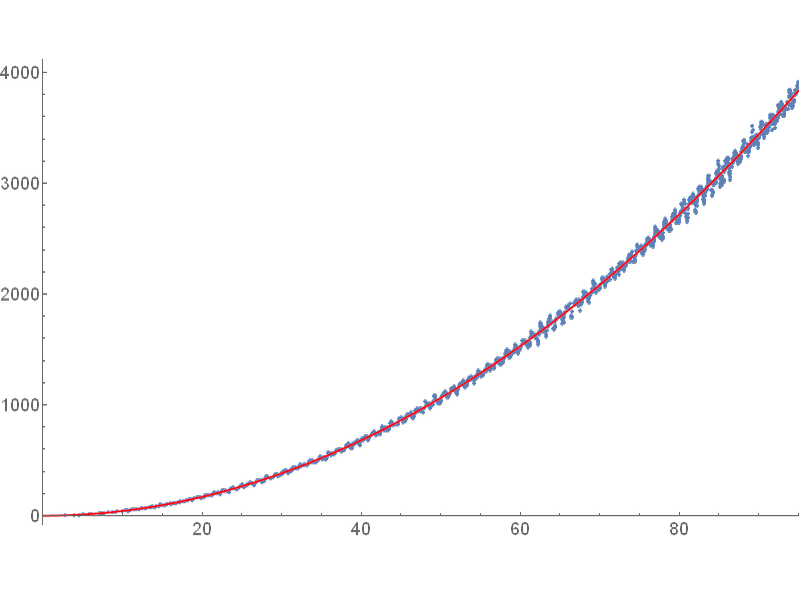
\includegraphics[width=0.45\textwidth]{dndx}}%
        \hspace{8pt}%
        %
        \subfloat[][]{%
            \label{fig:dndx_mag}%
            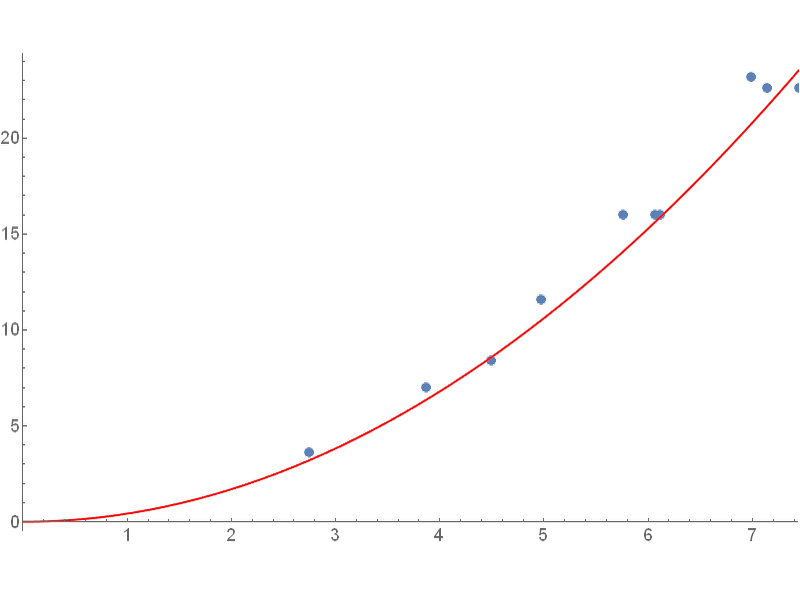
\includegraphics[width=0.45\textwidth]{dndx_mag}}%
        \hspace{8pt}%
        %
        \caption[]{Функция $\flatfrac{\Delta N}{\Delta \omega}$ (аргумент в относительных единицах), дискретная и непрерывная. Параметр $l_{max} = 100$. Размер окна~--- 5 относительных единиц. На \subref{fig:dndx_mag} увеличена область вблизи нуля. %
        } %
        \label{fig:dndx}%
    \end{figure}

    Более детально вопрос непосредственного получения $\flatfrac{\Delta N}{\Delta \omega}$ описан в \autoref{sec:getting_plank_formula}.

    Итак, мы показали, что асимптотически $\flatfrac{\Delta N}{\Delta \omega} \sim \omega^2$, причем данное соответствие имеет место уже при совсем небольших значениях $\omega$. Это, в свою очередь, доказывает справедливость формулы Планка и в случае сферических резонаторов. На \autoref{fig:plank} изображена кривая спектральной плотности энергии по дискретным данным с наложенной на нее классической непрерывной кривой. Как и ожидалось, кривые совпадают.
    %
    \begin{figure}[h]
        \centering
        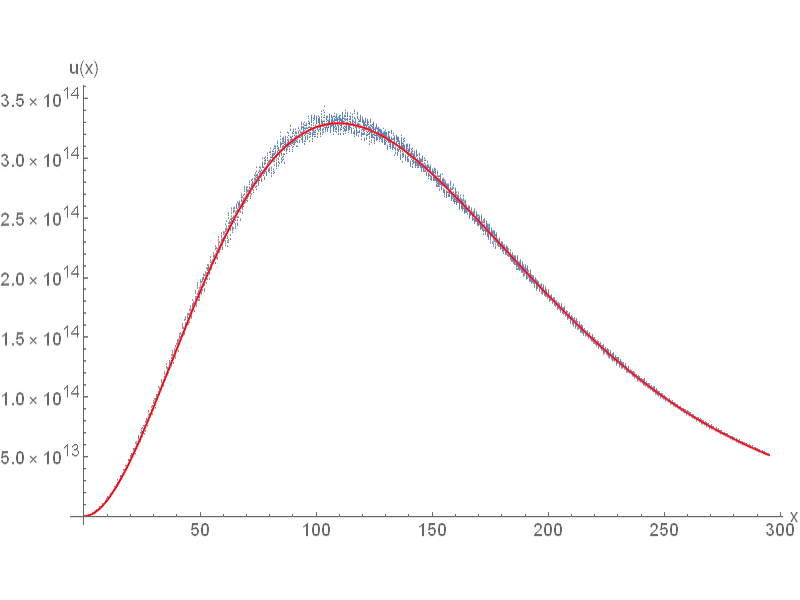
\includegraphics[width=0.5\textwidth]{plank}
        \caption[]{Планковская кривая, практическая (дискретная, построенная на данных \autoref{fig:dndx}; параметр $l_{max}$ увеличен до $300$) и теоретическая (непрерывная). Единицы относительные.}
        \label{fig:plank}
    \end{figure}
